\chapter{Landasan Teori}
\label{chap:teori}

\section{CodeIgniter}
\label{sec:codeigniter} 

CodeIgniter adalah sebuah \textit{framework} untuk membangun situs web menggunakan PHP. Tujuan utamanya adalah untuk mempercepat pembuatan proyek dengan menyediakan \textit{library} yang lengkap untuk fungsi-fungsi yang umum digunakan, serta antarmuka yang sederhana dan struktur yang logis untuk mengakses \textit{library} tersebut \cite{codeigniter}.

\begin{figure}[H]
	\centering  
	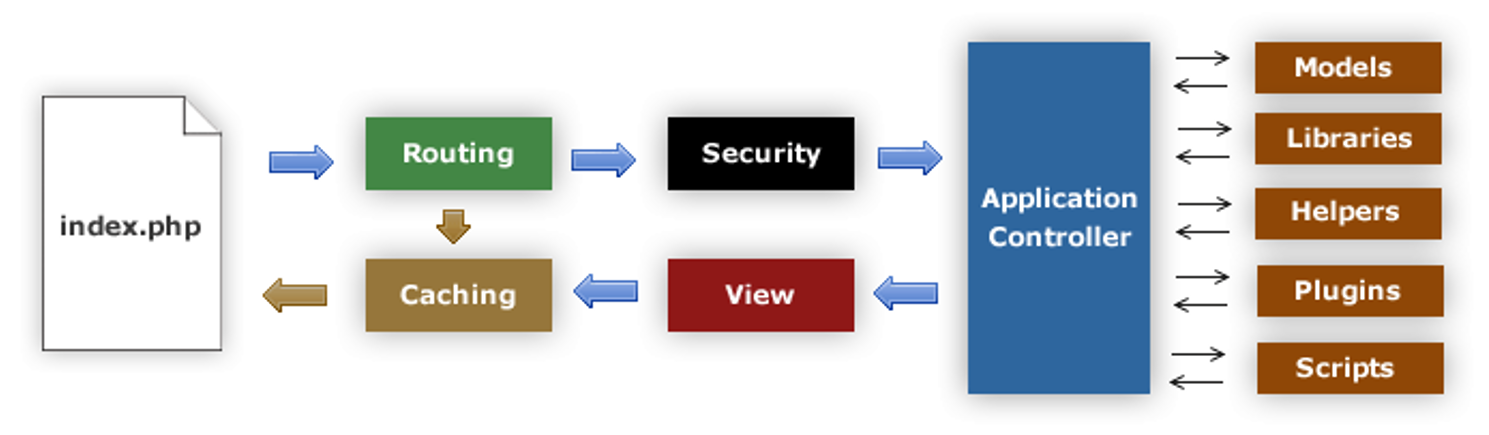
\includegraphics[scale=0.3]{ci-flowchart}  
	\caption[\textit{Flow Chart} CodeIgniter]{\textit{Flow Chart} CodeIgniter} 
	\label{fig:ciflowchart} 
\end{figure} 

Gambar~\ref{fig:ciflowchart} mengilustrasikan bagaimana data mengalir pada sistem CodeIgniter.

\begin{enumerate}
	\item \textit{File} index.php berfungsi sebagai \textit{front controller}, menginisialisasi \textit{resource} utama untuk menjalankan CodeIgniter.
	\item Router meneliti \textit{request} HTTP dan menentukan apa yang harus dilakukan.
	\item Jika terdapat \textit{file} \textit{cache}, maka langsung dikirimkan ke \textit{browser}.
	\item Sebelum \textit{controller} dimuat, seluruh \textit{request} HTTP dan data dari user disaring terlebih dahulu untuk keamanan.
	\item \textit{Controller} memuat \textit{model}, \textit{library} utama, dan  \textit{resource} lainnya yang diperlukan.
	\item \textit{View} akhir lalu dikirim ke browser untuk dilihat. \textit{Cache} akan dibuat terlebih dahulu bila diaktifkan. 
\end{enumerate}

\subsection{Model-View-Controller}
\label{subs:cimvc} 
CodeIgniter menggunakan pola arsitektur MVC (\textit{Model-View-Controller}) sebagai dasarnya. MVC memisahkan proses logika aplikasi dari presentasi. Dengan demikian, halaman web dapat memuat sedikit \textit{script} karena presentasinya terpisah dari \textit{scripting} PHP.

\subsubsection{Model}
\textit{Model} merepresentasikan struktur data. Biasanya \textit{model} memiliki fungsi-fungsi yang membantu dalam mengambil, memasukkan, dan memperbarui informasi pada \textit{database}. Pada CodeIgniter, \textit{model} adalah sebuah kelas yang mengekstensi \verb|CI_Model| dan terletak di direktori \verb|application/models/|.

\begin{lstlisting}[language=php, caption=Contoh \textit{model}, label=kode:cimodel]
class Blog_model extends CI_Model {

        public $title;
        public $content;
        public $date;

        public function get_last_ten_entries()
        {
                $query = $this->db->get('entries', 10);
                return $query->result();
        }

        public function insert_entry()
        {
                $this->title    = $_POST['title']; // please read the below note
                $this->content  = $_POST['content'];
                $this->date     = time();

                $this->db->insert('entries', $this);
        }

        public function update_entry()
        {
                $this->title    = $_POST['title'];
                $this->content  = $_POST['content'];
                $this->date     = time();

                $this->db->update('entries', $this, array('id' => $_POST['id']));
        }

}
\end{lstlisting}

Kode \ref{kode:cimodel} merupakan contoh sebuah kelas \textit{model} pada CodeIgniter. Kelas tersebut mengekstensi \verb|CI_Model| dan memiliki fungsi untuk mengambil, memasukkan, dan memperbarui \textit{database}.
	
\subsubsection{View}
\textit{View} adalah informasi yang ditampilkan kepada pengguna. Pada CodeIgniter, \textit{view} merupakan sebuah halaman web atau sebagian dari halaman web yang terletak di direktori \verb|application/view/|.

\begin{lstlisting}[language=php, caption=Contoh \textit{view}, label=kode:ciview]
<html>
<head>
        <title>My Blog</title>
</head>
<body>
        <h1>Welcome to my Blog!</h1>
</body>
</html>
\end{lstlisting}

Kode \ref{kode:ciview} merupakan contoh sebuah \textit{view}. \textit{View} pada CodeIgniter harus dipanggil melalui \textit{Controller} dan tidak pernah dipanggil secara langsung.
	
\subsubsection{Controller}
\textit{Controller} adalah perantara dari \textit{model} dan \textit{view}, serta \textit{resource} lainnya yang diperlukan untuk memproses \textit{request} HTTP dan menghasilkan sebuah halaman web. Pada CodeIgniter, \textit{controller} adalah sebuah kelas yang mengekstensi \verb|CI_Controller| dan terletak di direktori \verb|application/controllers/|.

\begin{lstlisting}[language=php, caption=Contoh \textit{controller}, label=kode:cicontroller]
<?php
class Blog extends CI_Controller {

        public function index()
        {
                echo 'Hello World!';
        }

        public function comments()
        {
                echo 'Look at this!';
        }
}
\end{lstlisting}

Kode \ref{kode:cimodel} merupakan contoh sebuah kelas \textit{controller} pada CodeIgniter. Kelas tersebut mengekstensi \verb|CI_Controller| dan memiliki fungsi \verb|index()| dan \verb|comments()|. Fungsi \verb|index()| akan dipanggil secara otomatis jika tidak ada fungsi lain yang dipanggil. 

\begin{lstlisting}[language=php, caption=Contoh memuat \textit{model} dan menampilkan \textit{view}, label=kode:cimodelview]
<?php
class Blog_controller extends CI_Controller {

        public function blog()
        {
                $this->load->model('blog');

                $data['query'] = $this->blog->get_last_ten_entries();

                $this->load->view('blog', $data);
        }
}
}
\end{lstlisting}

Pada CodeIgniter, \textit{model} dan \textit{view} hanya dapat dimuat melalui controller. Pada contoh kode \ref{kode:cimodelview}, fungsi \verb|blog()| pada \textit{controller} memuat \textit{model} untuk mengambil data dari \textit{database}, lalu menampilkan \textit{view} yang memuat data tersebut. 

\subsection{URL CodeIgniter}
\label{subs:ciurl}

URL pada CodeIgniter menggunakan \textit{segment-based approach} yang dirancang untuk lebih mudah dibaca oleh \textit{search engine} dan manusia. Berikut ini adalah contoh sebuah URL pada CodeIgniter:
\begin{center}
    \verb|example.com/class/function/ID|    
\end{center}
\begin{itemize}
	\item Bagian pertama, \verb|class| merepresentasikan kelas \textit{controller} yang akan dipanggil.
	\item Bagian kedua,  \verb|function| merepresentasikan fungsi yang akan dipanggil.
	\item Bagian ketiga dan seterusnya, \verb|ID| merepresentasikan variabel yang akan digunakan.
\end{itemize}

\section{Twig}
\label{sec:twig}

Twig adalah sebuah \textit{template engine} untuk PHP. Sebuah \textit{template} Twig memuat \textit{variable} atau \textit{expression} yang nantinya akan diubah menjadi \textit{value} saat template dievaluasi, serta \textit{tag} yang mengontrol logika template \cite{twig}.

\begin{lstlisting}[language=php, caption=Contoh template Twig, label=kode:twig]
<!DOCTYPE html>
<html>
    <head>
        <title>My Webpage</title>
    </head>
    <body>
        <ul id="navigation">
        
            <li><a href="{{ item.href }}">{{ item.caption }}</a></li>
        
        </ul>

        <h1>My Webpage</h1>
        {{ a_variable }}
    </body>
</html>
\end{lstlisting}

Kode \ref{kode:twig} merupakan contoh sebuah template Twig. Terdapat dua jenis \textit{delimiter}, yaitu \verb|| dan \verb|{{ ... }}|. \textit{Delimiter} \verb|| digunakan untuk menjalankan \textit{statement} seperti \verb|for| dan \verb|if|, sementara \textit{delimiter} \verb|{{ ... }}| digunakan untuk menampilkan nilai dari \textit{variable} atau \textit{expression}.

\section{Shell Script}
\label{sec:shell}
\textit{Shell} adalah sebuah program pada sistem operasi Unix yang menerima perintah tertulis dan mengirimnya ke sistem operasi untuk dijalankan. Pada umumnya, perangkat Linux menggunakan program bernama Bourne Again SHell (Bash) sebagai \textit{shell}. Bash merupakan program yang disempurnakan dari \textit{shell} Unix pertama yang diciptakan oleh Steve Bourne \cite{linux}. 

\textit{Shell script} adalah sebuah \textit{file} yang menyimpan rangkaian perintah. \textit{Shell} akan membaca \textit{file} tersebut dan menjalankan rangkaian perintah seperti jika perintah tersebut dimasukkan secara langsung pada \textit{command line}. Keunikan dari \textit{shell} adalah kemampuannya sebagai \textit{command line interface} dan sebagai  \textit{scripting language interpreter}. Artinya, hal yang dapat dilakukan melalui \textit{command line} dapat dilakukan sebagai \textit{script}, dan hal yang dapat dilakukan sebagai \textit{script} dapat dilakukan melalui \textit{command line}.

\section{PDF.js}
\label{sec:pdfjs} 
PDF.js adalah sebuah library JavaScript yang berfungsi untuk menampilkan \textit{file} Portable Document Format (PDF) menggunakan HTML5 \textit{Canvas} \cite{pdfjs}. PDF.js terdiri dari 3 \textit{layer}:

\begin{itemize}
	\item \textit{\textbf{Core}} merupakan bagian dimana proses \textit{parse} dan \textit{interpret} dilakukan terhadap \textit{binary} PDF.
	\item \textit{\textbf{Display}} mengambil \textit{layer} \textit{core} sebagai API yang lebih mudah digunakan untuk menampilkan PDF dan mengambil informasi lainnya dari sebuah dokumen.
	\item \textit{\textbf{Viewer}} membangun \textit{layer} \textit{display} sebagai halaman website dengan \textit{user interface} yang dapat ditampilkan di browser.
\end{itemize}

\begin{lstlisting}[language=php, caption=Contoh kode untuk menggunakan PDF.js, label=kode:pdfjs]
<!DOCTYPE html>
<html>
    <iframe src="/web/viewer.html?file=sample.pdf"></iframe>
</html>
\end{lstlisting}

Salah satu cara untuk menampilkan \textit{file} PDF menggunakan PDF.js adalah dengan \textit{embed} layer \textit{viewer} yang sudah tersedia melalui \verb|web/viewer.js| pada sebuah \verb|iframe|. Kode \ref{kode:pdfjs} merupakan contoh kode \textit{embed} PDF.js untuk menampilkan sebuah file PDF contoh \verb|sample.pdf|.

\section{Ace}
\label{sec:ace} 
Ace adalah sebuah library JavaScript yang berfungsi sebagai \textit{code editor}.
Ace memiliki fitur-fitur yang dapat ditemukan di \textit{code editor} pada umumnya \cite{ace}. Berikut ini merupakan beberapa fitur utama dari Ace: 

\begin{itemize}
    \item \textit{Syntax highlighting} untuk lebih dari 110 bahasa pemrograman.
    \item \textit{Indent} dan \textit{outdent} otomatis.
    \item Kemampuan \textit{cut}, \textit{copy}, dan \textit{paste}.
    \item \textit{Drag and drop} teks menggunakan mouse.
\end{itemize}

Berikut ini adalah beberapa kelas yang terdapat pada Ace:

\begin{itemize}
    \item \verb|Ace| \\ Kelas utama yang digunakan mempersiapkan Ace pada browser. Salah satu fungsi yang dimiliki:
        \begin{itemize}
            \item \texttt{edit(String | DOMElement el)} \\ \textit{Embed} Ace pada elemen yang disediakan.
        \end{itemize}
    \item \verb|Anchor| \\ Menangani posisi \textit{pointer} pada dokumen.
    \item \verb|BackgroundTokenizer| \\ Bekerja di latar belakang untuk melakukan tokenisasi pada dokumen saat ini dan menyimpan baris yang sudah ditokenisasi sebagai \textit{cache}.
    \item \verb|Document| \\ Menyimpan teks dari dokumen. 
    \item \verb|EditSession| \\ Menyimpan seluruh \textit{state} untuk \verb|Editor| dan menyediakan cara untuk mengubahnya dengan mudah. Beberapa fungsi yang dimiliki:
        \begin{itemize}
            \item \verb|getMode()| \\ Mengembalikan mode \textit{syntax highlighting} editor yang sedang digunakan.
            \item \verb|setMode()| \\ Mengubah mode \textit{syntax highlighting} editor.
        \end{itemize}
    \item \verb|Editor| \\ \textit{Entry point} utama untuk seluruh kegunaan Ace. Beberapa fungsi yang dimiliki:
        \begin{itemize}
            \item \verb|getReadOnly()| \\ Mengembalikan \verb|true| jika editor sedang menggunakan pengaturan \textit{read-only}.
            \item \verb|getTheme()| \\ Mengembalikan alamat tema editor yang sedang digunakan.
            \item \verb|getValue()| \\ Mengembalikan isi teks editor.
            \item \verb|setReadOnly(Boolean readOnly)| \\ Mengubah pengaturan \textit{read-only}.
            \item \verb|setTheme(String style)| \\ Mengubah tema editor.
            \item \verb|setValue(String val, Number cursorPos)| \\ Mengubah isi teks editor.
        \end{itemize}
    \item \verb|Range| \\ Mengindikasi sebuah daerah pada editor.
    \item \verb|Scrollbar| \\ Menangani \textit{scrollbar} editor.
    \item \verb|Search| \\ Menangani seluruh operasi pencarian teks pada dokumen.
    \item \verb|Selection| \\ Menyimpan posisi kursor dan seleksi teks pada editor.
    \item \verb|TokenIterator| \\ Menyediakan fungsi untuk membaca dokumen sebagai aliran token.
    \item \verb|Tokenizer| \\ Menerima sejumlah aturan dan membuat \verb|Tokenizer|.
    \item \verb|UndoManager| \\ Menangani fungsi \textit{undo} pada editor.
    \item \verb|VirtualRenderer| \\ Menggambar tampilan yang terlihat di layar.
\end{itemize}


\begin{lstlisting}[language=php, caption=Contoh kode untuk menggunakan Ace, label=kode:ace]
<!DOCTYPE html>
<html>
<head>
<title>ACE in Action</title>
</head>
<body>

<div id="editor">
function foo(items) {
    var x = "All this is syntax highlighted";
    return x;
}
</div>
    
<script src="/ace-builds/src-noconflict/ace.js" type="text/javascript" charset="utf-8"></script>
<script>
    var editor = ace.edit("editor");
    editor.setTheme("ace/theme/monokai");
    editor.session.setMode("ace/mode/javascript");
</script>
</body>
</html>
\end{lstlisting} 

Kode \ref{kode:ace} merupakan contoh kode untuk menempatkan editor Ace pada sebuah elemen \verb|div| dengan id \verb|editor|. Terdapat berbagai konfigurasi pada Ace, pada contoh ini digunakan tema \textit{monokai} dan mode \textit{syntax highlighting} untuk JavaScript.




